\documentclass[11pt, titlepage, dvipdfmx, twoside]{jarticle}
\linespread{1.1}
%\documentclass[11pt,dvipdfmx,twoside]{jarticle}
%%%%%%%%%%%%%%%%%%%%%%%%%%%%%%%%%%%%%%%%%%%%%%%%%%%%%%%%%%%%%%%%%%%%%%%%%%%%%%
% style definitions
%
% following setting makes 3cm spaces for top and bottom, and
% 2.5cm spaces for left and right
%
                                         % default setting
\setlength{\oddsidemargin}{22pt}         % 62pt
\setlength{\evensidemargin}{22pt}        % 62pt
\setlength{\headheight}{12pt}            % 12pt
\setlength{\textheight}{662pt}           % 592pt
\setlength{\marginparsep}{10pt}          % 10pt
\setlength{\footskip}{30pt}              % 30pt
\setlength{\hoffset}{-13pt}              % 0pt
\setlength{\paperwidth}{597pt}           % 597pt
\setlength{\topmargin}{20pt}             % 20pt
\setlength{\headsep}{25pt}               % 25pt
\setlength{\textwidth}{427pt}            % 327pt
\setlength{\marginparwidth}{106pt}       % 106pt
\setlength{\marginparpush}{5pt}          % 5pt
\setlength{\voffset}{-37pt}              % 0pt
\setlength{\paperheight}{845pt}          % 845pt


% 1 inch = 2.54 cm = 72.27 pt

\renewcommand{\baselinestretch}{1.20}

%%%%%%%%%%%%%%%%%%%%%%%%%%%%%%%%%%%%%%%%%%%%%%%%%%%%%%%%%%%%%%%%%%%%%%%%%%%%%%
\usepackage{amsfonts}
\usepackage{amssymb}
\usepackage{amsmath}
\usepackage[dvipdfmx]{graphicx}
\usepackage{framed}
\usepackage{url}
\usepackage{color}

%%%%%%%%%%%%%%%%%%%%%%%%%%%%%%%%%%%%%%%%%%%%%%%%%%%%%%%%%%%%
%\newcommand{\project}{{\tt mol-infer/Cyclic\_improved}}
\newcommand{\project}{{\tt mol-infer/Cyclic}}
\newcommand{\secref}[1]{第\ref{sec:#1}節}
\newcommand{\tabref}[1]{表\ref{tab:#1}}
\newcommand{\figref}[1]{図\ref{fig:#1}}
%%%%%%%%%%%%%%%%%%%%%%%%%%%%%%%%%%%%%%%%%%%%%%%%%%%%%%%%%%%%

\title{\huge Module 2におけるニューラルネットワーク学習の手順}
\author{\project}
\begin{document}
\makeatletter 
\let\c@lstlisting\c@figure
\makeatother
\西暦
\date{\today}
\maketitle
\thispagestyle{empty}
\tableofcontents
\clearpage
\pagenumbering{arabic}


\section{はじめに}
本稿では,本プロジェクト (\project) における Module 2の手順を解説する.

与えられた化学グラフの集合を $D_\pi=\{G_1,G_2,\dots,G_p\}$,
化学グラフを特徴ベクトルに変換する写像を $f$ とする.
${\mathcal F}(D_\pi)\triangleq\{f(G_1),f(G_2),\dots,f(G_p)\}$と定義する. 
また, 注目する化学的性質を $\pi$ と書くことにする.
この $\pi$ は,たとえば沸点,燃焼熱,水分配係数など様々である.
Module 2 の入力と出力は以下の通りである.

\begin{oframed}
\begin{description}
\item[入力:] 特徴ベクトルの集合 ${\mathcal F}(D_\pi)=\{x_1,x_2,\dots,x_p\}$,
  各化合物 $G_i\in D_\pi$ もといその特徴ベクトル $x_i=f(G_i)\in{\mathcal F}(D_\pi)$
  が化学的性質 $\pi$ に関して持つ値の集合 $\{a(x_1),a(x_2),\dots,a(x_p)\}$,
  ニューラルネットワークの各種パラメータの値(隠れ素子の個数など).
\item[出力:] 入力で指定された構造を持ち,${\mathcal F}(D_\pi)$における
  「多くの」特徴ベクトル $x\in {\mathcal F}(D_\pi)$に
  対して
  化学的性質の値 $a(x)$ を「良く」推定するようなニューラルネットワーク.
\end{description}
\end{oframed}
出力の具体的な中身は,学習されたニューラルネットワークにおける
各枝の重みと各ノードのバイアスである.

本稿の構成は以下の通りである.
\begin{itemize}
\item \secref{preparation}: 基本的な用語,およびパッケージのファイル構成の説明.
\item \secref{quick}: 簡単な実行例.
\item \secref{io}: プログラムの入出力に関する詳細.
\end{itemize}

%%%%%%%%%%%%%%%%%%%%%%%%%%%%%%%%%%%%%%%%%%%%%%%%%%%%%%%%%%%%
\newpage
\section{準備}
\label{sec:preparation}

\subsection{用語の説明}
\paragraph{特徴ベクトル.}
各元素の種類の原子数等の化学物質を説明する数値,
あるいはグラフの直径等の化学物質のグラフ表現のトポロジーに基づいて
計算される数値のベクトル.

\paragraph{人工ニューラルネットワーク (ANN).}
人工ニューラルネットワーク (artifician neural network, ANN),
または単にニューラルネットワーク (NN) とは,機械学習で最も確立した手法の1つである.これらは入力ベクトルに基づいて値を予測するために用いられる.この冊子では,ニューラルネットワークへの入力は,化合物の特徴ベクトルであり,出力は特定の化学的性質の予測値である.

本プロジェクトで用いるのはフィードフォーワード型のニューラルネットワークであり,
これは非巡回有向グラフによって表すことができる.\figref{sample}に例を示す.

\begin{figure}[h!]
  \centering
  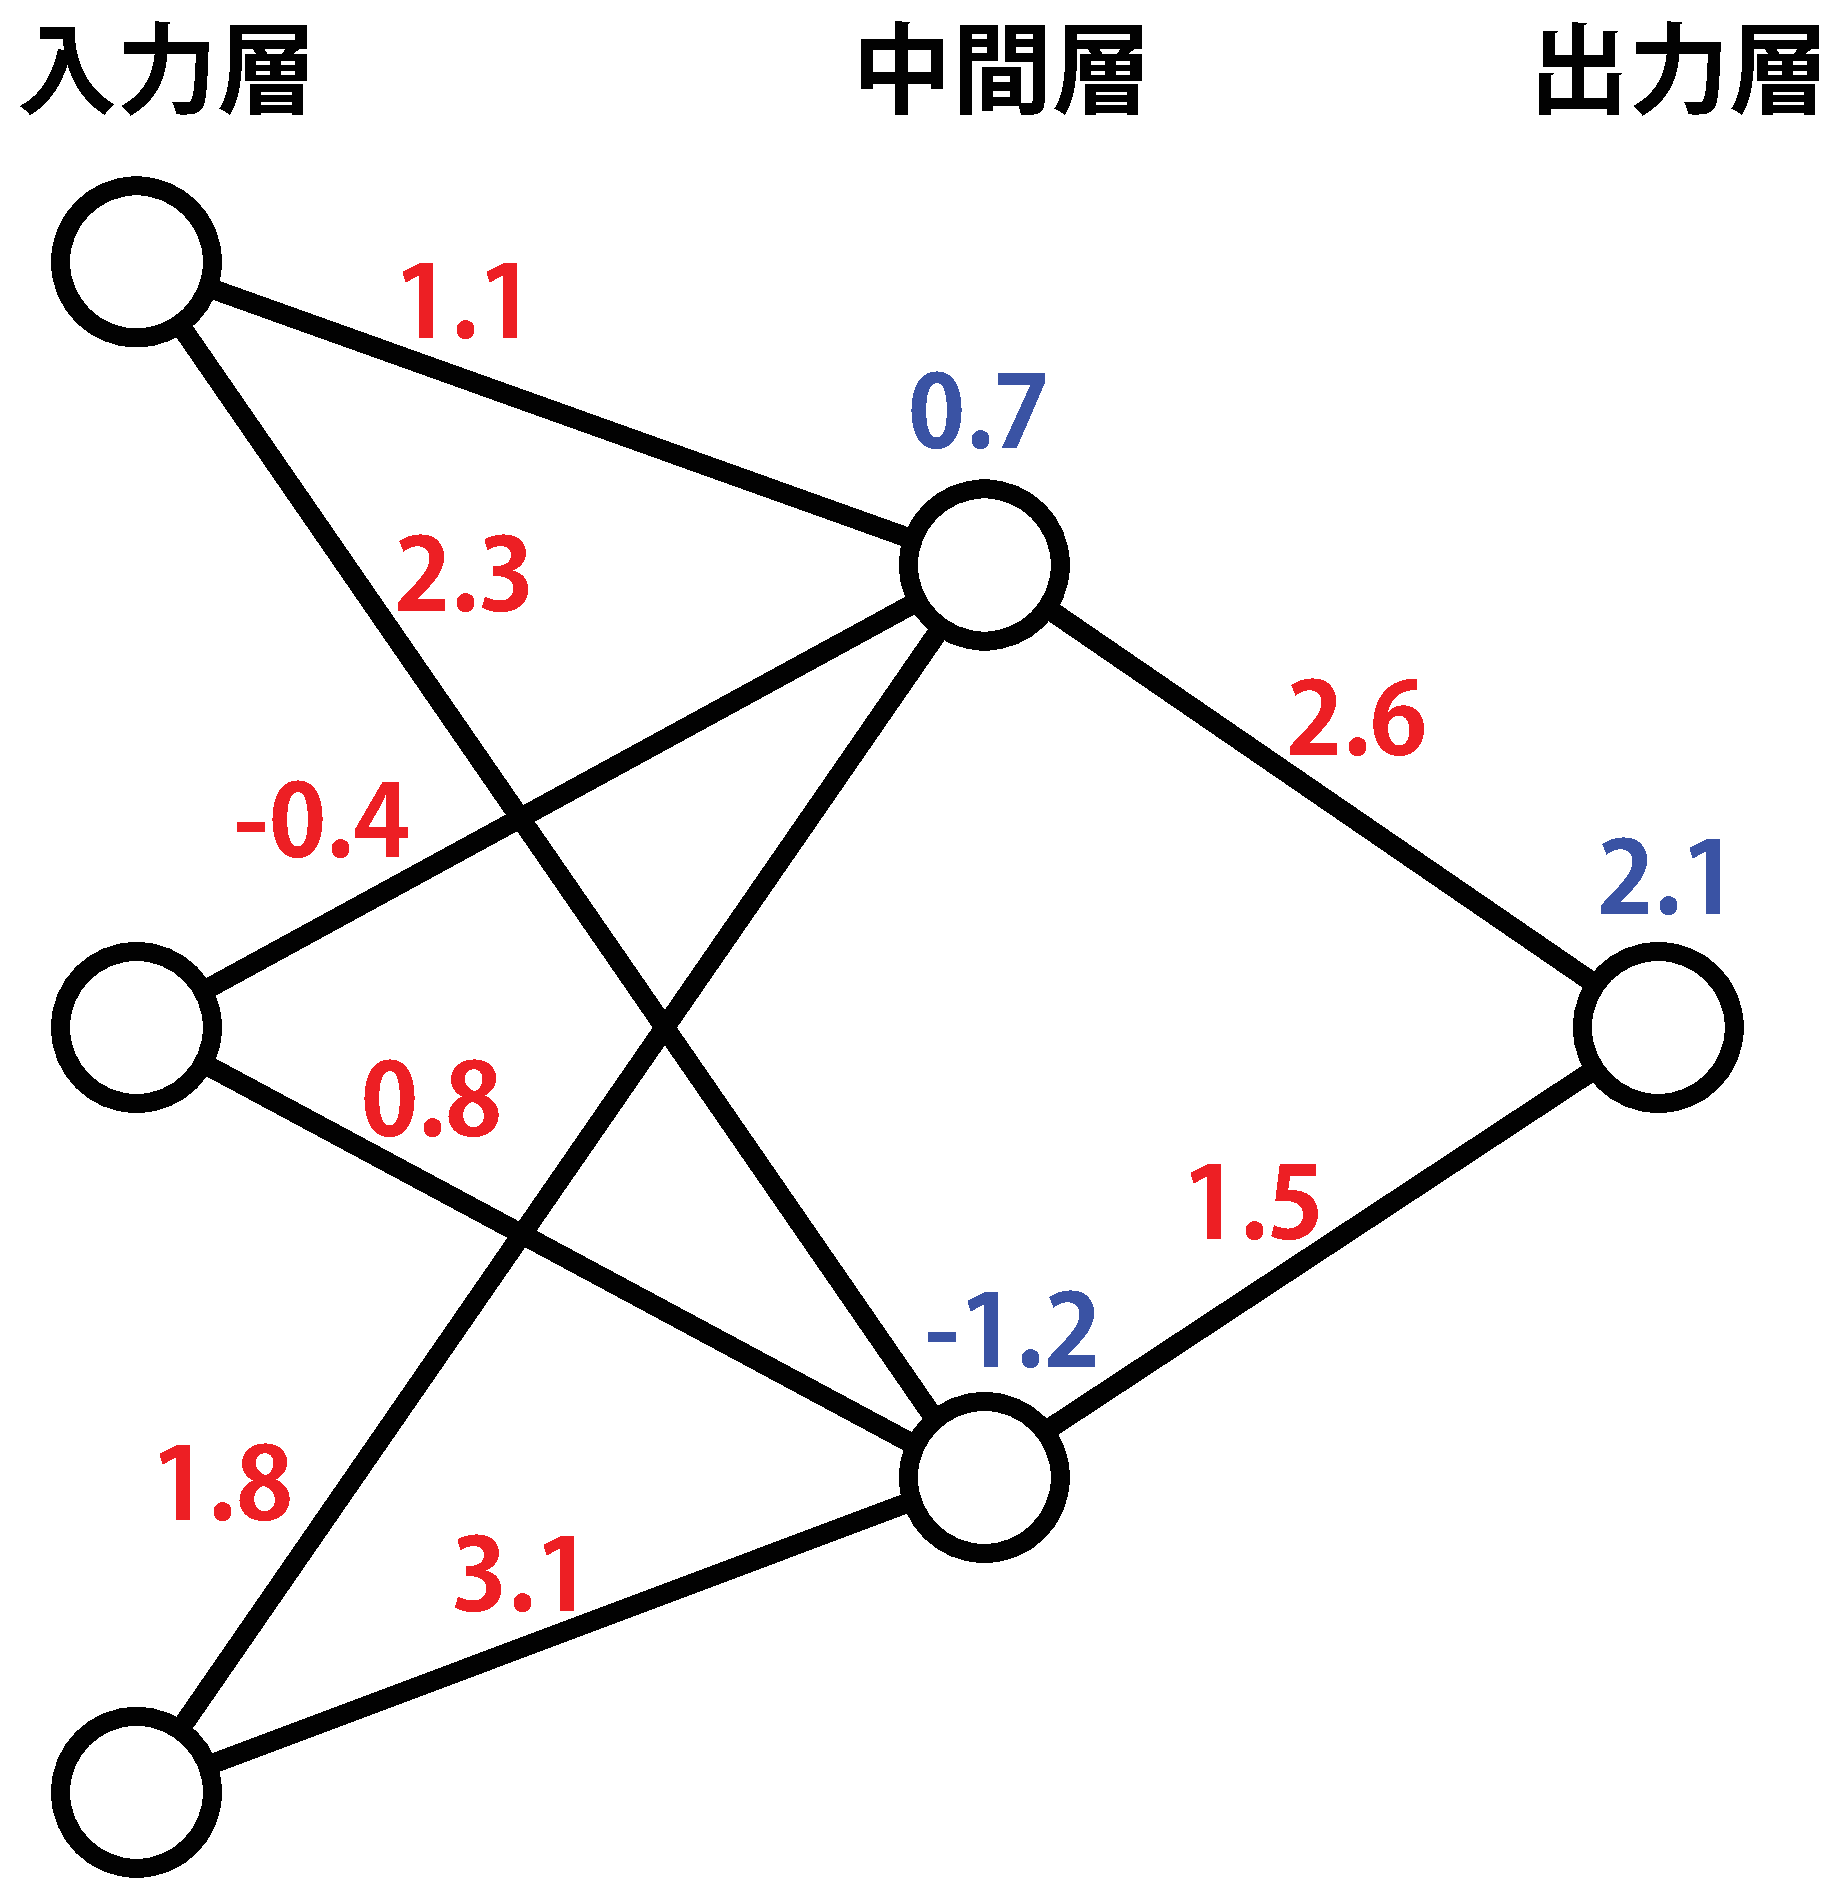
\includegraphics[width = 0.4 \textwidth]{./fig/ANN_sample_jp}
  \caption{ニューラルネットワークの具体例.
  赤色の数値が重み,青色の数値がバイアスを表している.枝はすべて左から右に向いている.}
  \label{fig:sample}
\end{figure}

\paragraph{入力層,隠れ層,出力層.}
人工ニューラルネットワークの多層パーセプトロンモデルを仮定する.このモデルでは,ニューラルネットワークはいくつかの層で構成されている.最初の層は入力層で,入力層は場合によっては特徴ベクトルから数値データを得るため,特徴ベクトルの要素と同じ数のノードがある.次に数値は隠れ層を介して伝播される.隠れ層は1つの層の計算が次の層への入力として用いられる.最後に出力層が入力ベクトルに基づいた予測値を与える.

\figref{sample}では,入力層は3つのノードを持つ.
したがって入力する特徴ベクトルは3次元のものでなければならない.
また1つの隠れ層を有し,この隠れ層は2つのノードを持つ.
そして出力層は1つのノードを持つ.

\paragraph{重み.}
ニューラルネットワークでは,ノード間を接続する枝(有向枝)にはそれぞれ数値が割り当てられ,
その値を重みと呼ぶ.入力層から出力層への値の伝播には,これらの重みに基づく計算が含まれている.

\figref{sample}では,枝の重みは赤によって示される.


\paragraph{バイアス.}
ニューラルネットワークの隠れ層の各ノードにはバイアスと呼ばれる数値が割り当てられている.この数値は重みと共に,入力ベクトルに基づいて出力値を計算する過程で使用される.

\figref{sample}では,ノードのバイアスは青によって示される.

\paragraph{活性化関数.}
活性化関数はニューラルネットワークの各ノードに割り当てられており,
与えられた入力ベクトルから出力値を計算する際に用いられる.
特に各ノードの出力値は,重み付けされた対応する枝の重みと
前の層からのノードの出力の線形結合を入力として与えられた活性化関数の値である.

本プロジェクトでは,隱れ層の各ノードの活性化関数として
Rectified Linear-Unit (ReLU) 関数を限定して用いる.
これは次の Module 3 (この Module 2 で学習したニューラルネットワークに基づいた化合物推定)
では,活性化関数が ReLU であることを仮定しているからである. 

\medskip

%ニューラルネットワークは,与えられた入力ベクトルと目標値の組に基づいて
%重みとバイアスの組を計算する.このプロセスは一般に「学習」と呼ばれる.


\subsection{ファイル構成}
パッケージに含まれるファイルとその役割は\tabref{files}の通りである.
\begin{table}[h!]
  \centering
  \caption{Module 2 のパッケージに含まれるファイルとその役割}
  \label{tab:files}
  \begin{tabular}{lcll}
  \hline
  \bf ファイル名 &\ \ & \multicolumn{2}{l}{\bf 役割}\\
  \hline
  \verb|mol-infer_ANN.py| && \multicolumn{2}{l}{NNを学習するためのPythonスクリプト}\\
  &&\multicolumn{2}{l}{\bf (Module 3に進むにはこのスクリプトの実行が必要)}\\
  &&\multicolumn{2}{l}{$\bullet$使用する非標準ライブラリ: {\tt numpy, pandas, scikit-learn}}\\
  \hline
  \verb|predict_values.py| && \multicolumn{2}{l}{学習したNNを用いて}\\
  &&\multicolumn{2}{l}{化学的性質の値を推定するための補助的なPythonスクリプト}\\
  &&\multicolumn{2}{l}{(このスクリプトの実行は必ずしも必要ではない)}\\
  &&\multicolumn{2}{l}{$\bullet$使用する非標準ライブラリ: {\tt numpy, pandas}}\\
  \hline
  \multicolumn{4}{l}{\tt Manual\_Module\_2\_Cyclic\_jp.pdf}\\
  \multicolumn{4}{l}{\tt Manual\_Module\_2\_Cyclic\_jp.tex}\\
  %\multicolumn{4}{l}{\tt Manual\_Module\_2\_Cyclic\_improved\_jp.pdf}\\
  %\multicolumn{4}{l}{\tt Manual\_Module\_2\_Cyclic\_improved\_jp.tex}\\
  \multicolumn{4}{l}{\tt fig/ANN\_sample\_jp.eps}\\
  &&\multicolumn{2}{l}{マニュアルのPDF,\LaTeX ソースファイル}\\
  &&\multicolumn{2}{l}{および画像ファイル(日本語版)}\\
  \hline
  \multicolumn{4}{l}{\tt Manual\_Module\_2\_Cyclic\_en.pdf}\\
  \multicolumn{4}{l}{\tt Manual\_Module\_2\_Cyclic\_en.tex}\\
  %\multicolumn{4}{l}{\tt Manual\_Module\_2\_Cyclic\_improved\_en.pdf}\\
  %\multicolumn{4}{l}{\tt Manual\_Module\_2\_Cyclic\_improved\_en.tex}\\
  \multicolumn{4}{l}{\tt fig/ANN\_sample\_en.eps}\\
  &&\multicolumn{2}{l}{マニュアルのPDF,\LaTeX ソースファイル}\\
  &&\multicolumn{2}{l}{および画像ファイル(英語版)}\\
  \hline
  \multicolumn{4}{l}{\bf BP (boiling point; 沸点) に関するデータファイル~\cite{pubchem}}\\
  \multicolumn{2}{l}{\tt data/BP.sdf} & \multicolumn{2}{l}{化合物に関するSDFファイル.Module 2 では直接取り扱わない}\\
  \multicolumn{2}{l}{\tt data/BP\_fv.csv} & \multicolumn{2}{l}{Module 1 に{\tt BP.sdf}を入力して生成した特徴ベクトル}\\
  \multicolumn{2}{l}{\tt data/BP\_value.csv} & \multicolumn{2}{l}{化合物のBP値を記したファイル}\\
  \multicolumn{2}{l}{\tt data/BP\_ANN.LOG} & \multicolumn{2}{l}{{\tt BP\_fv.csv, BP\_value.csv}から成るデータセットに対して}\\
  &&\multicolumn{2}{l}{{\tt mol-infer\_ANN.py}を実行し,学習したときのログ出力}\\
  \multicolumn{4}{l}{\tt data/BP\_ANN\_biases.txt} \\
  \multicolumn{4}{l}{\tt data/BP\_ANN\_weights.txt} \\
  &&\multicolumn{2}{l}{学習されたNNにおける各ノードのバイアス,}\\
  &&\multicolumn{2}{l}{および各枝の重み}\\
  \hline
  \end{tabular}
\end{table}

\newpage

\begin{table}[t!]
  \centering
  (\tabref{files}の続き)
  \begin{tabular}{lcll}
  \hline
  \bf ファイル名 &\ \ & \multicolumn{2}{l}{\bf 役割}\\
  \hline
  \multicolumn{4}{l}{\bf HC (heat of combustion; 燃焼熱) に関するデータファイル~\cite{pubchem}}\\
  \multicolumn{2}{l}{\tt data/HC.sdf} & \multicolumn{2}{l}{化合物に関するSDFファイル.Module 2 では直接取り扱わない}\\
  \multicolumn{2}{l}{\tt data/HC\_fv.csv} & \multicolumn{2}{l}{Module 1 に{\tt HC.sdf}を入力して生成した特徴ベクトル}\\
  \multicolumn{2}{l}{\tt data/HC\_value.csv} & \multicolumn{2}{l}{化合物のHC値を記したファイル}\\
  \multicolumn{2}{l}{\tt data/HC\_ANN.LOG} & \multicolumn{2}{l}{{\tt HC\_fv.csv, HC\_value.csv}から成るデータセットに対して}\\
  &&\multicolumn{2}{l}{{\tt mol-infer\_ANN.py}を実行し,学習したときのログ出力}\\
  \multicolumn{4}{l}{\tt data/HC\_ANN\_biases.txt} \\
  \multicolumn{4}{l}{\tt data/HC\_ANN\_weights.txt} \\
  &&\multicolumn{2}{l}{学習されたNNにおける各ノードのバイアス,}\\
  &&\multicolumn{2}{l}{および各枝の重み}\\
  \hline
  \multicolumn{4}{l}{\bf KOW (log Kow; オクタノール/水分配係数) に関するデータファイル~\cite{pubchem}}\\
  \multicolumn{2}{l}{\tt data/KOW.sdf} & \multicolumn{2}{l}{化合物に関するSDFファイル.Module 2 では直接取り扱わない}\\
  \multicolumn{2}{l}{\tt data/KOW\_fv.csv} & \multicolumn{2}{l}{Module 1 に{\tt KOW.sdf}を入力して生成した特徴ベクトル}\\
  \multicolumn{2}{l}{\tt data/KOW\_value.csv} & \multicolumn{2}{l}{化合物のKOW値を記したファイル}\\
  \multicolumn{2}{l}{\tt data/KOW\_ANN.LOG} & \multicolumn{2}{l}{{\tt KOW\_fv.csv, KOW\_value.csv}から成るデータセットに対して}\\
  &&\multicolumn{2}{l}{{\tt mol-infer\_ANN.py}を実行し,学習したときのログ出力}\\
  \multicolumn{4}{l}{\tt data/KOW\_ANN\_biases.txt} \\
  \multicolumn{4}{l}{\tt data/KOW\_ANN\_weights.txt} \\
  &&\multicolumn{2}{l}{学習されたNNにおける各ノードのバイアス,}\\
  &&\multicolumn{2}{l}{および各枝の重み}\\
  \hline
  \multicolumn{4}{l}{\bf MP (melting point; 融点) に関するデータファイル~\cite{pubchem}}\\
  \multicolumn{2}{l}{\tt data/MP.sdf} & \multicolumn{2}{l}{化合物に関するSDFファイル.Module 2 では直接取り扱わない}\\
  \multicolumn{2}{l}{\tt data/MP\_fv.csv} & \multicolumn{2}{l}{Module 1 に{\tt MP.sdf}を入力して生成した特徴ベクトル}\\
  \multicolumn{2}{l}{\tt data/MP\_value.csv} & \multicolumn{2}{l}{化合物のMP値を記したファイル}\\
  \multicolumn{2}{l}{\tt data/MP\_ANN.LOG} & \multicolumn{2}{l}{{\tt MP\_fv.csv, MP\_value.csv}から成るデータセットに対して}\\
  &&\multicolumn{2}{l}{{\tt mol-infer\_ANN.py}を実行し,学習したときのログ出力}\\
  \multicolumn{4}{l}{\tt data/MP\_ANN\_biases.txt} \\
  \multicolumn{4}{l}{\tt data/MP\_ANN\_weights.txt} \\
  &&\multicolumn{2}{l}{学習されたNNにおける各ノードのバイアス,}\\
  &&\multicolumn{2}{l}{および各枝の重み}\\
  \hline
  \end{tabular}

\end{table}


%%%%%%%%%%%%%%%%%%%%%%%%%%%%%%%%%%%%%%%%%%%%%%%%%%%%%%%%%%%%
\clearpage
\section{クイックスタート}
\label{sec:quick}

\paragraph{ニューラルネットワークの学習.}

次のコマンドを入力すれば,
\verb|data/BP_fv.csv|を特徴ベクトル,
\verb|data/BP_value.csv|を化学的性質(この場合はBP,すなわち沸点)の値
とするようなデータセットに対し,
2つの隠れ層を持ち,それぞれの隠れ層における
ノード数を20, 10とするようなニューラルネットワークが学習され,
そのニューラルネットワークにおける各枝の重みは\verb|output_weights.txt|,
各ノードのバイアスは
\verb|output_biases.txt|
にそれぞれ出力される.

\begin{oframed}
{\small
\verb|$ python mol-infer_ANN.py data/BP_fv.csv data/BP_value.csv output 20 10|
\hfill $(\clubsuit)$}
\end{oframed}

学習されたニューラルネットワークの{\bf 重みおよびバイアスに関するファイルは,Module 3でも使用}する.


\paragraph{化学的性質の値の推定.}
学習したニューラルネットワークを用いて,
化合物の化学的性質の値を推定することができる.

次のコマンド\footnote{一行目の最後のバックスラッシュ $\backslash$ は,実際に入力するときには改行してはならないことを示す.}を入力すれば,
学習済ニューラルネットワーク(枝の重みは\verb|output_weights.txt|,ノードのバイアスは\verb|output_biases.txt|に保持されている)を用いて,\verb|data/BP_fv.csv|に記述された特徴ベクトル(に対応する化合物)の化学的性質の値が推定され,その結果は\verb|predicted.txt|に出力される.

\begin{oframed}
  {\small
\begin{verbatim}
$ python predict_values.py output_weights.txt output_biases.txt \
    data/BP_fv.csv predicted.txt
\end{verbatim}
}
  \end{oframed}

\begin{itemize}
\item 化学的性質の値を推定したい化合物の特徴ベクトルは,Module 1の特徴ベクトル生成器を用いて生成することができる.
\item 上のコマンドは,さらに上のコマンド$(\clubsuit)$で\verb|data/BP_fv.csv|を
  特徴ベクトルとしたデータセットから学習したニューラルネットワークに関する \verb|output_weights.txt|および \verb|output_biases.txt|を用いるものとみなせば,
  データセット自身の化学的性質の値を推定していることになる.
\item この推定機能は補助的なものに過ぎず,Module 3以降で使用することはない.
\end{itemize}


\section{プログラムの入出力に関する詳細}
\label{sec:io}

\subsection{入力}
\subsubsection{特徴ベクトル}
特徴ベクトルは,我々が{\bf FV形式}と呼ぶフォーマットに基づく
csvファイルに記述されている必要がある.
Module 1の特徴ベクトル生成器は
化合物に関するSDFファイルから
FV形式のcsvファイルを生成するため,
当該生成器を用いて生成されたファイルを用いれば問題はない.

以下,FV形式の記述ルールを簡単に記しておく.
\begin{oframed}
  {\small
\begin{verbatim}
CID,n,cs,ch,nsH
244,8,6,2,8
307,10,6,4,8
657014,11,7,1,18
16704,9,9,0,10
\end{verbatim}
}
\end{oframed}
\begin{itemize}
\item FV形式では先頭行に記述子の名前をコンマ区切りで記述する.
\item ただし最初の記述子は CID(化合物識別番号)でなければならない.CIDの値が学習に用いられることはない.CIDは識別のためのみに用いられる.
\item 上記の例では,\verb|n|(水素を除く原子の個数),\verb|cs|(コアサイズ),\verb|ch|(コアハイト),\verb|nsH|(水素原子の個数)と四つの記述子が定められている.
\item 二行目以降に,一つの行に一つの化合物のCIDおよび特徴ベクトルを,コンマ区切りで記述する.
  したがって各化合物は,4次元の特徴ベクトルで表されることになる.
\item 化合物がCIDの昇順あるいは降順に並んでいる必要はない.
\end{itemize}


\subsubsection{化学的性質の値}
化学的性質の値は,CIDと値を羅列したcsvファイルに記述されなければならない.
\begin{oframed}
  {\small
\begin{verbatim}
CID,a
307,11.2
244,-0.5
657014,98.124
16704,-12.8
117,5.3
\end{verbatim}
}
\end{oframed}
\begin{itemize}
\item {\bf 先頭行は\verb|CID,a|でなければならない.}
\item 二行目以降に,一つの行に一つの化合物のCIDおよび化学的性質の値を
  コンマ区切りで記述する.
\item 化合物がCIDの昇順あるいは降順に並んでいる必要はない.
\end{itemize}
  
\subsection{実行}
\secref{quick}で示したとおり,
ニューラルネットワークを学習するには{\tt mol-infer\_ANN.py}を用いる.

\subsubsection{引数}
\secref{quick}で示したコマンドを再掲する.
\begin{oframed}
{\small
\verb|$ python mol-infer_ANN.py data/BP_fv.csv data/BP_value.csv output 20 10|
}
\end{oframed}
各引数には以下を指定する.
\begin{itemize}
\item 第1引数: 特徴ベクトルに関するcsvファイル
\item 第2引数: 化学的性質の値に関するcsvファイル
\item 第3引数: 学習されたニューラルネットワークの重み・バイアスを書き込むファイルの名前
\item 第4引数以降: 隠れ層(中間層)のノードの個数
\end{itemize}

引数を与えずに実行すれば(もしくは引数が適切に与えられなかった場合),
引数に関する説明が英語で出力される.
\begin{oframed}
  {\small
\begin{verbatim}
$ python mol-infer_ANN.py 
\end{verbatim}
  }
  \end{oframed}


引数が適切に与えられると,ニューラルネットワークの学習が始まる.

5分割交差検定が行われ,試験集合に対して最も高い決定係数 (${\rm R}^2$値) を
実現するニューラルネットワークが採用され,
その重みとバイアスが,ファイルに出力される.
上記のコマンドの場合,そのファイルの名前は第3引数で指定された\verb|output|に基づく,
\begin{itemize}
\item \verb|output_weights.txt|(重み)
\item \verb|output_biases.txt|(バイアス)
\end{itemize}
である.これら出力されたファイルは,Module 3 の実行に必要となる.


\paragraph{データセットに関する注意.}
データセットは,
\begin{itemize}
\item 特徴ベクトルに関するcsvファイル,および
\item 化学的性質の値に関するcsvファイル
\end{itemize}
の二つのファイルから構成されるが,
CID は前者ファイルに記されたものすべて,かつそれのみが計算の対象となる.
したがって,
\begin{center}
  {\bf 前者ファイルに記されたCIDは,
  すべて後者ファイルに記されていなければならない.}
\end{center}
しかし逆は成り立たなくともよい.
つまり,化学的性質の値に関するcsvファイルには,
特徴ベクトルのcsvファイルに記されていない,
「余計な」CIDに関する値が記されていても構わない.
そのような値は無視される.

\subsubsection{ハイパーパラメータの調整}
ニューラルネットワークの学習は{\tt scikit-learn}ライブラリ\footnote{\url{https://scikit-learn.org/stable/}}
における{\tt MLPRegressor}を用いて行われる.
\verb|mol-infer_ANN.py|の133行目以降で\verb|MLPRegressor|インスタンスの初期化が行われるが,
ハイパーパラメータの調整はここで行うことができる.
一部のパラメータを以下のように設定している.
\begin{itemize}
\item \verb|activation|: \verb|'relu'| {\color{red}{\bf 注意:} 学習されたニューラルネットワークを Module 3 以降で用いるには, \verb|'relu'| (ReLU関数) でなければならない.}
\item \verb|alpha|: $10^{-5}$
\item \verb|early_stopping|: \verb|False|
\item \verb|hidden_layer_sizes|: 実行時に引数で指定した個数に基づく
\item \verb|max_iter|: $10^{10}$
\item \verb|random_state|: 1
\item \verb|solver|: \verb|'adam'|
\end{itemize}

\subsection{出力}
ふたたび以下のコマンドを取り上げ,
その実行によって得られる出力について説明する.
\begin{oframed}
{\small
\verb|$ python mol-infer_ANN.py data/BP_fv.csv data/BP_value.csv output 20 10|
}
\end{oframed}

\subsubsection{標準出力}
上記コマンドを実行すると端末(標準出力)に計算過程が出力される.
この出力例がパッケージ内のファイル\verb|data/BP_ANN.LOG|に記されている.
\begin{oframed}
  {\small
\begin{verbatim}
src/preparation/BP_fv.csv contains 181 vectors for 107 (=CID+106) features.
src/preparation/BP_value.csv contains 230 target values.
n range = [5,30]
a range = [31.5,470.0]
#instances = 181
#features = 106

D1: train 144, test 37
training time: 3.187196731567383
R2 score train = 0.9935319077425955
R2 score test = 0.7855694851759929
R2 score all = 0.9599908495442584
MAE score train = 3.8570127089010384
MAE score test = 19.756408746147212
MAE score all = 7.10716548999556

D2: train 145, test 36
training time: 5.0139079093933105
R2 score train = 0.9930416804444452
R2 score test = 0.6390572625074291
R2 score all = 0.9339056805642507
MAE score train = 3.7281172621746888
MAE score test = 27.996544836634186
MAE score all = 8.554986834995363

D3: train 145, test 36
training time: 4.264358758926392
R2 score train = 0.9961346879653636
R2 score test = 0.8566979846124056
R2 score all = 0.9637772344809027
MAE score train = 2.870368503215682
MAE score test = 22.925217956024927
MAE score all = 6.8591783391335435

D4: train 145, test 36
training time: 2.9935202598571777
R2 score train = 0.9909067339023991
R2 score test = 0.8390994594153819
R2 score all = 0.9669036994338265
MAE score train = 4.470398694611737
MAE score test = 18.691072072382227
MAE score all = 7.298819918919681

D5: train 145, test 36
training time: 4.9648661613464355
R2 score train = 0.9946933391220482
R2 score test = 0.8479544758088942
R2 score all = 0.9574271159388575
MAE score train = 3.352287445970431
MAE score test = 21.80973582058148
MAE score all = 7.023382150312958
0.9935319077425955 0.7855694851759929 0.9599908495442584 3.187196731567383
0.9930416804444452 0.6390572625074291 0.9339056805642507 5.0139079093933105
0.9961346879653636 0.8566979846124056 0.9637772344809027 4.264358758926392
0.9909067339023991 0.8390994594153819 0.9669036994338265 2.9935202598571777
0.9946933391220482 0.8479544758088942 0.9574271159388575 4.9648661613464355
Average time = 4.08476996421814
Average R2 test score = 0.7936757335040208
Average MAE test score = 22.235795886354005
  \end{verbatim}        
}
\end{oframed}

\begin{itemize}
\item  冒頭で特徴ベクトルの個数,特徴数が出力される.また水素を除く原子数(特徴\verb|n|)の最小値と最大値 (\verb|n range|,上の例では5と30),および化学的性質(この場合はBP; 沸点)の値の
最小値と最大値(\verb|a range|,上の例では31.5と470.0)が出力される.
\item 続いて5分割交差検定における5回の学習の概要が出力される.
\item 最後に平均計算時間,(試験集合に対する)平均R$^2$値,
(試験集合に対する)平均MAE値が出力される.
\item 上記の例では,3回目の学習で得られたニューラルネットワークが
最も高い(試験集合に対する)R$^2$値を達成しているので(0.856697$\dots$),
当該ニューラルネットワークにおける枝重みが\verb|output_weights.txt|,
ノードのバイアスが\verb|output_biases.txt|に出力される.
\item なおこれらファイルのコピーを,それぞれ
\verb|data/BP_ANN_weights.txt|,\verb|data/BP_ANN_biases.txt|
として同封している.
\end{itemize}


\subsubsection{枝の重み}
\verb|mol-infer_ANN.py|が出力する枝重みファイルの書式について説明する.

簡単のため,\figref{sample}に示したニューラルネットワークが学習されたとする.
このニューラルネットワークの枝重みは以下のようにファイルに出力される.

\begin{oframed}
{\small
\begin{verbatim}
3 2 1
1.1 2.3
-0.4 0.8
1.8 3.1
2.6
1.5
\end{verbatim}
}
\end{oframed}
\begin{itemize}
\item 最初の行はニューラルネットワークの構造,つまり入力層のノード数,各隠れ層のノード数,最後に出力層のノード数である.
\item 2行目以降は枝重みの値である.各行は1つのノードから出る枝重みの値を示す.
\end{itemize}


\subsubsection{ノードのバイアス}
同じく,\verb|mol-infer_ANN.py|が出力するノードの
バイアスに関するファイルの書式について説明する.

やはり簡単のため,\figref{sample}に示したニューラルネットワークが学習されたとする.
このニューラルネットワークのノードのバイアスは以下のようにファイルに出力される.

\begin{oframed}
{\small
\begin{verbatim}
0.7
-1.2
2.1
\end{verbatim}
}
\end{oframed}
1行につき1つのノードのバイアスの値が示されている.
入力層のノードにはバイアスの値がないことに注意せよ.


\begin{thebibliography}{9}
\bibitem{pubchem} HSDB in PubChem \url{https://pubchem.ncbi.nlm.nih.gov} (2021年2月1日 アクセス確認)
\end{thebibliography}


\end{document}
%%%%%%%%%%%%%%%%%%%%%%%%%%%%%%%%%%%%%%%%%%%%%%%%%%%%%%%%%%%%
%%%%%%%%%%%%%%%%%%%%%%%%%%%%%%%%%%%%%%%%%%%%%%%%%%%%%%%%%%%%
%%%%%%%%%%%%%%%%%%%%%%%%%%%%%%%%%%%%%%%%%%%%%%%%%%%%%%%%%%%%

